\documentclass{tudphygp_eng}
\usepackage{tudphymd,mhchem}
\usepackage{lmodern}

\versuch{Elektronenbeugung (Electron Diffraction)}{EB}
\author{M.~Kreller}
\bearbeitet{A.~Otto, engl. S.~Saager}

\begin{document}
\maketitle

\section{Description of the Experiment}
This experiment deals with the wave aspect of the electron. A focused electron beam will be scattered at a graphite target and will be visualized at a phosphorescent screen.
 
In analogy to x-ray diffraction the wavelength of the electron will be determined by \textsc{Bragg}'s law.
\begin{figure}[htb]
\centering
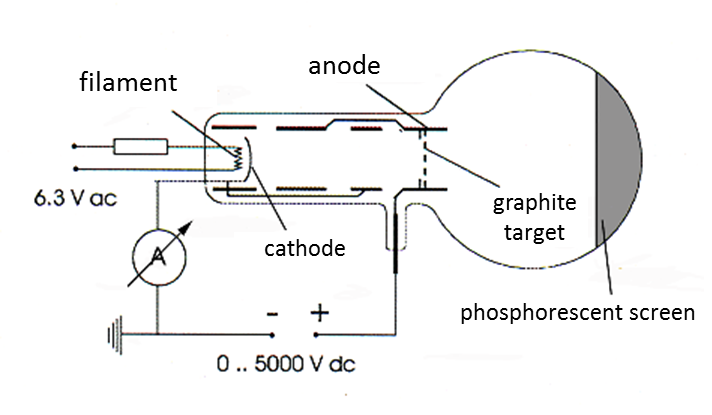
\includegraphics[width=0.8\textwidth]{schema_en}
\caption{Experimental setup.\label{schema}}
\end{figure}
The experimental setup is sketched up in Fig. \ref{schema}. A cathode in an evacuated glass tube will be heated up to temperature of several hundred \SI{}{^\circ C}. Due to the increase in temperature a small part of the electrons reach the energy threshold for overcoming the potential barrier and leaving the cathode material into vacuum.    
Because of the positive voltage of the anode these electrons will be accelerated. The generated electron beam will be focused by passing alternating charged tubular electrodes. The electron beam hits a target of polycrystalline graphite at the end of the setup and will be scattered at this. Behind the target a screen with a phosphorescent coating is placed. By hitting of electrons the screen luminesces and the collision point is visualized.

\subsection{Preparations for Experiment}
\begin{figure}[htb]
\centering
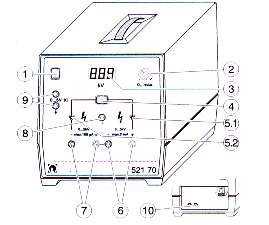
\includegraphics[width=9cm]{netzteil}
\caption{ power supply: (1) on/off-switch; (2) potentiometer for direct continuous setting of the output voltage or for setting the upper limit during external control of the output voltage by input connector(9);
(3) digital display for output voltage; (4) switch for output activation (right position: output (6); left position: output (7); center position: outputs (6) and (7) connected in series);
(5) LED for control of activated outputs; (6) or (7) outputs for power extraction controlled by potentiometer (2) or by external voltage input (9) (Output voltage is current limited and ungrounded); (8) ground connector, galvanic connected to protective ground; (9) input for external control of the output voltage, which has to be smaller than the limit set point of potentiometer (2); (10) (rear panel)
\SI{6,3}{V}-output for power supply of the filament, load limit: \SI{2}{A}.\label{netzteil}}
\end{figure}
Connect the electron scattering tube to the power supply in the same manner as sketched in Fig. \ref{schema}. The power supply is illustrated in Fig. \ref{netzteil}. The contact sockets (10) for the filament are placed on rear panel. Supply a positive voltage to the anode. Connect the cathode in series with a multimeter to the contact socket (6) labeled with "-". Connect the socket (6) to ground connector (8). The mulitmeter has to be adjusted to full scale \SI{2}{mA} DC. Turn down the high voltage potentiometer (2) to the lowest voltage. Switch on the power supply and turn up the voltage slowly. The current should be below \SI{0,2}{mA}.

\subsection{Experiment: The Wave aspect of the Electron}
Adjust different values for the acceleration voltage and measure the diameter $D$ of all visible rings by a vernier caliper. Estimate the width of the rings. The center of the glass sphere does not coincide with the center of the target. Calculate the distance between the target and the image on the phosphorescent screen by using Fig. \ref{korrektur} and calculate the scattering angle $2\,\theta$. Calculate the wavelength and plot in the momentum $p$ vs. the wavelength of the electrons. Determine the coefficient of proportionality and compare it with equation (\ref{B1}).
\begin{figure}[h]
\centering
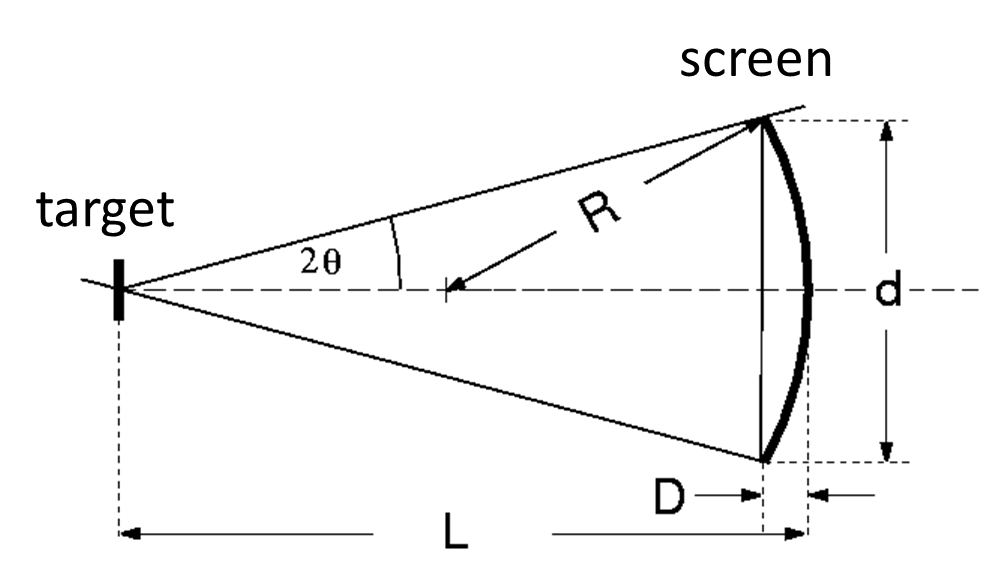
\includegraphics[width=10cm]{korrektur_en}
\caption{Correction of the distance between the image on the phosphorescent screen and the target. The values are $L=\SI{140}{mm}$ and $R=\SI{66}{mm}$. $R$ is the internal radius of sphere. The thickness of the glass is \SI{1,5}{mm}.
\label{korrektur}}
\end{figure}

\section{Theoretical Fundamentals}
\subsection{The Wave--Particle Duality}
Since the publication of \textsc{Albert Einstein}'s theory of relativity it is well known, that every energy $E$ is assigned to a mass $m$ according to the famous equation $E=m\,c^2$, with $c$ as the velocity of light. This interpretation has the consequence that also light is associated with mass. Since the work of \textsc{Max Planck} for the explanation of the black body radiation it is also known that the energy of electromagnetic radiation is related to the radiation frequency by the equation $E=h\nu$, with $h$ as the \textsc{Planck}'s constant. Because photons move with the velocity of light the photon momentum is given by

\begin{equation}
p=\frac{h\nu}{c}=\frac{h}{\lambda}\,\,.\label{B1b}
\end{equation}
In equation \ref{B1b} $ \lambda$ is the wavelength of light. The evidence for the particle behavior of photons was impressively shown by \textsc{Arthur Compton} in 1922 and the observed effect was named after him. If light shows simultaneously the characteristics of a wave as well as the characteristics of a particle, then the question arises, whether, conversely particles have wave properties.

\begin{figure}[htb]
\centering
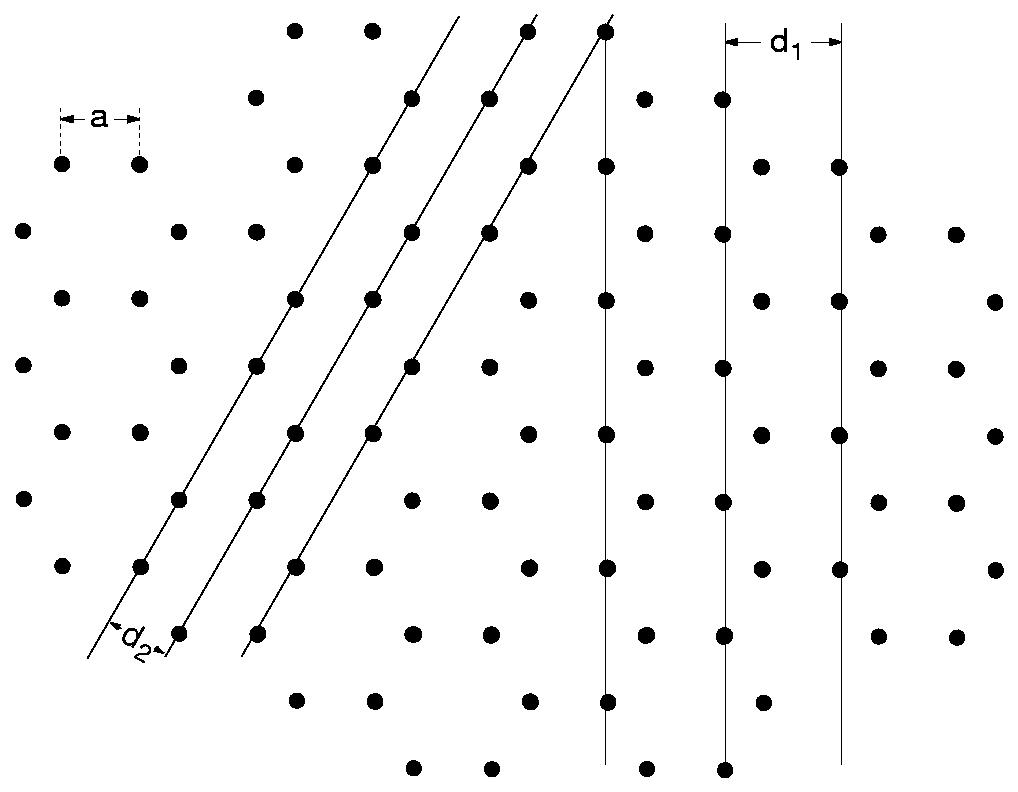
\includegraphics[width=8cm]{hexagonal}
\hspace{1cm}
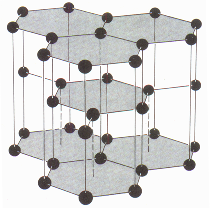
\includegraphics[width=5cm]{graphit}
\caption{Lattice planes of graphite. The right part of the figure shows the three dimensional arrangement of atoms of graphite. The layer structure is highlighted. The hatched planes of the figure are illustrated separately in the left part. 
\label{hexagonal}}
\end{figure}

The idea was created by \textsc{de Broglie} in 1924 by establishing his famous equation. He postulated the same relation between momentum and wavelength for a particle by following equation, which has a similar appearance as eq. (\ref{B1b}):
\begin{equation}
p=\frac{h}{\lambda}\,\,.\label{B1}
\end{equation}
Let us assume a moving particle with the velocity $v$, in which is $v\ll c$ for considering the nonrelativistic case only. Then the wavelength of the particle can be expressed by $\lambda=h/(mv)$ or based on the energy of the particle:
\begin{equation}
\lambda=\frac{h}{\sqrt{2\,m\,E}}\,\,.
\end{equation}
By passing the potential difference $U$ the electrons will be accelerate and get a kinetic energy $E$, which applies to:
\begin{equation}
E=\frac{p^2}{2\,m}=e\,U\,\,.
\end{equation}
In this equation $e$ is the elementary charge of electron. For the wavelength it becomes 
\begin{equation}
\lambda=\frac{h}{\sqrt{2\,m\,e\,U}}\,\,.
\end{equation}
Therefore a wavelength of \SI{2}{\AA} (typical distance between two lattice planes in graphite) corresponds to a voltage of $U=\SI{3,76}{kV}$.

The relation (\ref{B1}) was experimental proven by \textsc{Clinton J. Davisson} and \textsc{Lester H. Germer} in 1927. They used the duality of electromagnetic waves and particles by adapting the earlier known phenomenon of x-ray diffraction at crystal lattice to electrons.

\subsection{X-ray Diffraction}
In general diffraction phenomena only appear, when the wavelength is the same order of magnitude of the diffraction structure.  

For x-rays, which have a wavelength in the range of \SI{e-10}{m}, such a diffraction structure cannot be fabricated mechanically. So it is well suitable, that the distances in a crystal lattice are in same order of magnitude. Therefore crystals in their natural occurrence are perfect diffraction objects for x-rays. 
 
\begin{figure}[htb]
\centering
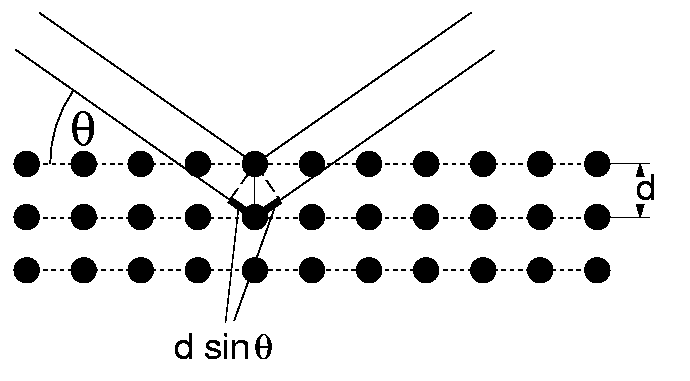
\includegraphics[width=10cm]{bragg}
\caption{\textsc{Bragg}'s law for constructive interference for x-rays during diffraction at a crystal lattice.\label{bragg}}
\end{figure}
In this experiment a graphite target will be used. Graphite consists of a plane stack with hexagonal symmetry (see Fig. \ref{hexagonal} right). These planes are also called basal planes. The left part of Fig. \ref{hexagonal} illustrates a basal planes in top view. The drawn lines mark planes, which are orthogonal to the basal planes. Two plane families $d_1$ and $d_2$ are highlighted. Such planes consisting of atoms of a crystal are also called lattice planes. 
X-rays guided onto a crystal lattice will be scattered elastically at the atoms of a lattice plane, or in simple words, they will be reflected at the plane. Reflected x-rays from adjacent planes can interfere with each other. This fact is schematically shown in Fig. \ref{bragg}. Constructive interference will appear, when the extra traveled length between two x-rays, which are scattered at the upper and underlying crystal plane, respectively, is a multiple of the wavelength. This is exactly the case, if

\begin{equation}
2 \,d\,\sin\theta=n\lambda\,\,.\label{B2}
\end{equation}

$d$ is the distance between the lattice planes, $n$ is the order of diffraction and $\lambda$ is the x-ray wavelength. This requirement is known as \textsc{Bragg}'s law. The process of reflecting x-rays at crystal planes will be called \textsc{Bragg} reflection.

\begin{figure}[htb]
\centering
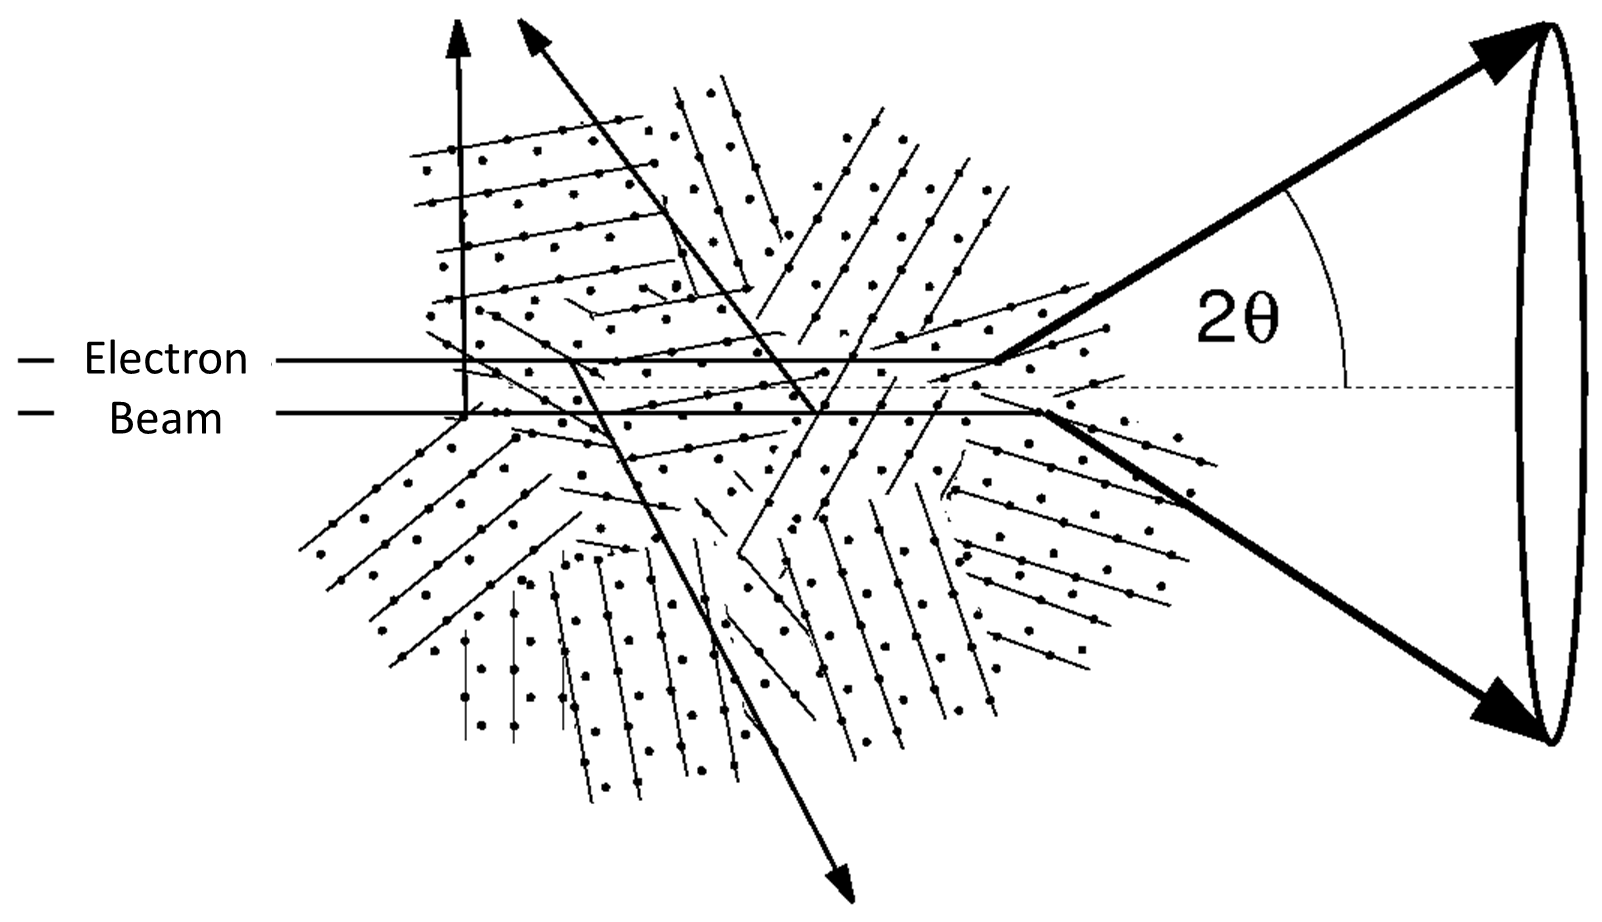
\includegraphics[width=10cm]{polycrystal3_en}
\caption{Diffraction of x-rays or electrons at a polycrystalline material.\label{polycrystal3}}
\end{figure}

Instead of a perfect infinitely extended crystal (so called single crystal) in this experiment a poly crystalline graphite layer will be used. Because it consists of small, arbitrarily oriented crystallites, certain lattice planes have an arbitrary orientation relative to the incident x-ray or electron beam. This correlation is illustrated in Fig. \ref{polycrystal3}. A certain lattice plane is highlighted but the figure is also correct for any other lattice planes. The reflection at an arbitrary lattice plane can occur in many different directions. But constructive interference will only be observed for a direction satisfying equation (\ref{B2}). Due to the arbitrary orientation of the crystallites in all spatial directions scattered x-rays with constructive interference will build up circular rings around the direction of the incident beam. For any other lattice plane analog rings with a different diameter will build up likewise. From equation (\ref{B2}) it follows an increasing ring diameter for a decreasing the distance between the lattice planes $d$. Which ring diameter would you expect?
Due to the large anisotropy of graphite his layer structure is retained also at polycrystalline material. Only the orientation of the crystallites within the layer is arbitrarily arranged. In this experiment the surface of the graphite target is approximately parallel to the basal planes. Therefore the electron beam has an orthogonal incident angle (see Fig. \ref{schema}) on this planes. It can be simply shown, that no reflection from this planes will occur in this geometrical configuration. Only planes, which are orthogonal to the basal planes, can cause reflections. From x-ray diffraction experiments it is known, from all possible lattice planes perpendicular to the basal plane only those two planes marked in Fig. \ref{hexagonal} can cause a visible reflection. 
If you use electrons instead of x-rays, you can test the \textsc{de-Broglie} relation (\ref{B1}). If electrons will not have wave properties, one would expect a complete diffuse scattering distribution with low dependence from the electron energy. However if electrons will show wave characteristics with a wavelength given by eq. (\ref{B1}), rings should be visible on the phosphorescent screen behind the target analogous to x-ray diffraction. In this case the radius of the rings has to be correlated to the wavelength, or in other words, correlated to the energy of the electrons.


%\section{Auswertung der Messergebnisse}


%Es konnten bis zu einer Spannung von 2.5~kV auf dem Leuchtschirm jeweils zwei Ringe beobachtet
%werden.
%Bei Spannungen unterhalb 2.5~keV sind die Ringe kaum noch zu erkennen. Die Durchmesser der Ringe
%wurden
%von 2.5~keV bis 5~keV in Schritten von 0.5~keV gemessen. Mit Ausnahme der Spannung $U$=2.5~keV
%wurden jeweils
%zwei Werte notiert, einer für den äusseren und einer für den inneren Rand des Ringes.

%Aus Abbildung \ref{korrektur} ergibt sich für den Abstand $D$ bei einem Durchmesser $d$ der
%beobachteten Ringe
%\begin{equation}
%D=R\Bigl[1-\sqrt{1-\Bigl(\frac{d/2}{R}\Bigr)^2}\,\,\Bigr]\,\,.
%\end{equation}
%Für den Winkel $\theta$ gilt
%\begin{equation}
%\tan(2\theta)=\frac{d}{2}\frac{1}{L-D}\,\,.
%\end{equation}
%Aus Abbildung \ref{hexagonal} folgt für die Ebenenabstände $d_1$=2.14~{\AA} und $d_2$=1.24~{\AA}.
%Damit lässt sich über Gleichung (\ref{B2}) die Wellenlänge berechnen.
%Die Tabellen \ref{Messwerte1} und \ref{Messwerte2} zeigen die gemessenen Werte und die daraus
%berechneten Wellenlängen.
%Der Fehler bestimmt sich hauptsächlich aus der Ungenauigkeit in der Bestimmung der
%Kreisdurchmesser.
%Da $D\ll L$ und $\theta \ll 1$,  gilt näherungsweise\nolinebreak ~$\lambda=2\,\,d_i\theta$ (i=1,2)
%und $\theta=d/(4\,L)$.
%Damit folgt für den Fehler von $\lambda$
%\begin{equation}
%\delta \lambda=\frac{d_i}{2\,L}\,\,\delta d\,\,,i=1,2\,\,.
%\end{equation}
%Für $\delta d$ wurde hier ein Wert von $\pm$0.5~mm für den kleineren Ring und $\pm$1~mm für den
%größeren
%Ring angenommen. Bei der Spannung $U$=2.5~keV wurde $\pm$1~mm bzw. $\pm$2~mm angenommen

%Aus den für $\lambda$ ermittelten Werten wurden Mittelwerte gebildet und gegen
%$1/\sqrt{E/\textrm{keV}}$ aufgetragen.
%Durch diese Werte wurde eine Ausgleichsgerade gelegt.
%Das Ergebnis zeigt Abbildung \ref{Gerade}. Für die Ausgleichsgerade $\lambda=a_0+a_1/\sqrt{E/keV}$
%ergibt sich $a_0$=0.00647$\pm 0.05$~{\AA} und $a_1$=0.38303$\pm 0.15$~{\AA}.
%Der Fehler lässt sich über die beiden Grenzgeraden, welche die Fehlerbalken der Messwerte
%gerade noch treffen, abschätzen. Der Messwert für die Spannung $U$=2.5~keV wurde dabei nicht
%verwendet.
%Nach Gleichung (\ref{B1}) ergibt sich für die Steigung der Geraden 0.388.
%Die übereinstimmung mit den gemessenen Werten ist erstaunlich gut.

%\begin{figure}[p]
%\centering
%\includegraphics[width=10cm,clip]{Gerade.eps}
%\caption{Ausgleichsgerade zur überprüfung der Bragg-Bedingung. Der Fehler wurde über die beiden
%Grenzgeraden ermittelt.
%Der letzte Messwert wurde dabei nicht verwendet.\label{Gerade}}
%\end{figure}


%\begin{table}[p]
%\centering
%\renewcommand{\arraystretch}{1.2}
%\begin{tabular}[htb]{|c|c|c|c|c|c|}\hline
%$U$/keV&$d_I$&$d_A$&$\bar{d}$&$\theta$/rad&$\lambda$/{\AA}\\ \hline
%5&20.6&23.9&22.3&0.0397&0.170$\pm0.002$\\
%4.5&22.8&26.7&24.8&0.0441&0.0189$\pm0.002$\\
%4&25.0&28.7&26.9&0.0478&0.0205$\pm0.002$\\
%3.5&26.2&29.4&27.8&0.0495&0.0212$\pm0.002$\\
%3&27.2&32.1&29.7&0.0528&0.0226$\pm0.002$\\
%2.5&-&-&34.2&0.0608&0.0260$\pm0.003$\\\hline
%\end{tabular}
%\caption{Gemessene Durchmesser und berechnete Wellenlängen für den kleineren Ring
%($d_1=21.4$~{\AA}).
%Die Größen $d_I$ und $d_A$ bezeichnen den inneren bzw. den äußeren Durchmesser der Ringe.
%Die Größe $\bar{d}$ bezeichnet den Mittelwert aus $d_I$ und $d_A$.
%\label{Messwerte1}}
%\end{table}



%\begin{table}[p]
%\centering
%\renewcommand{\arraystretch}{1.2}
%\begin{tabular}[htb]{|c|c|c|c|c|c|}\hline
%$U$/keV&$d_I$&$d_A$&$\bar{d}$&$\theta$/rad&$\lambda$/{\AA}\\ \hline
%5.0&37.6&42.9&40.3&0.0714&0.176$\pm0.002$\\
%4.5&41.3&46.4&43.9&0.0777&0.191$\pm0.002$\\
%4.0&42.7&48.2&45.5&0.0805&0.198$\pm0.002$\\
%3.5&45.6&52.6&49.1&0.0868&0.213$\pm0.002$\\
%3.0&49.2&56.1&52.7&0.0930&0.228$\pm0.003$\\
%2.5&-&-&54.1&0.0955&0.235$\pm0.003$\\\hline
%\end{tabular}
%\caption{Gemessene Durchmesser und berechnete Wellenlängen für den größeren Ring
%($d_1=1.23$~{\AA}).
%Die Größen $d_I$ und $d_A$ bezeichnen den inneren bzw. den äußeren Durchmesser der Ringe.
%Die Größe $\bar{d}$ bezeichnet den Mittelwert aus $d_I$ und $d_A$.
%\label{Messwerte2}}
%\end{table}

\frage{Calculate the distance between the planes in Fig. \ref{hexagonal} ! ($a=\num{1,425}$~{\AA})}
\frage{Which energy has an electron, whose wavelength has exactly the distances $d_1$ and $d_2$ in Fig. \ref{hexagonal}?}
\frage{The distance for the marked planes in the right part of Fig. \ref{hexagonal} is approximately \SI{3,4}{\AA}. With this information calculate the distance of neighboring atoms $a$ (Hint: The atomic weight of graphite is \SI{12}{g/mol} and the the density is \SI{2,25}{g/cm^3})!}
\frage{ Relativistic effects have to be considered only for energies higher than about $\num{0,1}\,m\,c^2$. Which acceleration voltage is required to generate such relativistic electrons?}
\frage{At diffraction experiments with visible light mostly mechanical fabricated gratings are used. Why this does not work with x-rays?}

\buch{Ott93}{G.~Otter, R.~Honecker}{Atome--Moleküle--Kerne, Band I Atomphysik}{Teubner-Ver\-lag}{Stuttgart 1993}
\buch{Ash01}{N.~W.~Ashcroft, N.~D.~Mermin}{Solid State Physics}{Harcourt Brace College Publ.}{1976}

\end{document}


